\documentclass{article}
\usepackage[T1]{fontenc}
\usepackage{lmodern}
\usepackage{graphicx}
\usepackage{amsmath,amssymb}
\usepackage[a4paper,margin=2cm]{geometry}
\usepackage[absolute,overlay]{textpos}
\setlength{\TPHorizModule}{1mm}
\setlength{\TPVertModule}{1mm}
\usepackage[indonesian]{babel}
\usepackage{hyperref}
\setlength{\emergencystretch}{2em}
% unit: Halaman 12

\begin{document}

% === Halaman 12 (llm) ===

\section*{3. Chosen-plaintext attack}

Kriptanalis dapat memilih plainteks sesuka hati untuk dienkripsikan, yaitu plainteks-plainteks yang lebih mengarahkan penemuan kunci, lalu mengirim plainteks ke sistem enkripsi. Asumsi: Penyerang memiliki akses ke sistem enkripsi

\vspace{5mm}

Diberikan: \[ P_1, C_1 = E_k(P_1), P_2, C_2 = E_k(P_2), \dots, P_i, C_i = E_k(P_i) \]
di mana kriptanalis dapat memilih diantara $P_1, P_2, \dots, P_i$

Deduksi: $k$ untuk mendapatkan $P_{i+1}$ dari $C_{i+1} = E_k(P_{i+1})$.

\vspace{5mm}

\begin{center}
\textbf{\color{red}Chosen-Plaintext Attack}
\end{center}

\vspace{10mm}

% deskripsi: Diagram ilustrasi serangan Chosen-Plaintext Attack yang melibatkan Alice, Eve (penyerang), dan Bob, menunjukkan bagaimana Eve memilih plainteks, mendapatkan cipherteks, dan menganalisisnya untuk menemukan kunci.
% bbox normalisasi: [0.2700, 0.6600, 0.7400, 0.9600]
\begin{textblock*}{98.70mm}(56.70mm,196.02mm)
\noindent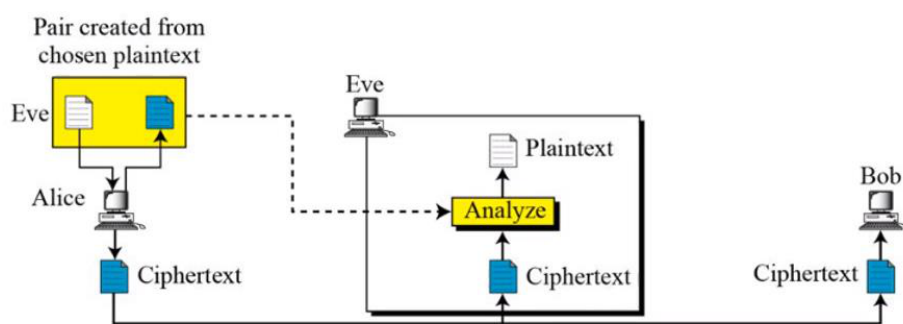
\includegraphics[width=98.70mm,height=89.10mm]{../../images/llm/page_012_img_01.png}%
\end{textblock*}

\end{document}
